\documentclass{beamer}
\usetheme{metropolis} % Use the metropolis theme




% Add tikz and pgfplots packages
\usepackage{tikz, pgfplots}
\usetikzlibrary{positioning}

% For clicking references
\usepackage{hyperref}

% For better horizontal lines
\usepackage{booktabs}

% For better referencing
\usepackage{cleveref}

\usepackage{graphicx}


\usepackage{amsmath}

\usepackage{wasysym}

% Define custom pastel colors
\definecolor{pastelRed}{RGB}{255, 105, 97}   % A soft pastel red
\definecolor{pastelBlue}{RGB}{119, 158, 203} % A muted pastel blue
\definecolor{pastelYellow}{RGB}{255, 223, 0} % A gentle pastel yellow
\definecolor{lightGray}{RGB}{211, 211, 211}  % A light gray for subtitles and less emphasized text

% Apply the custom colors
\setbeamercolor{palette primary}{bg=black, fg=white}
\setbeamercolor{palette secondary}{bg=lightGray, fg=black}
\setbeamercolor{palette tertiary}{bg=black, fg=white}
\setbeamercolor{titlelike}{parent=palette primary, fg=black}
\setbeamercolor{subtitle}{fg=lightGray}
\setbeamercolor{structure}{fg=black} % For itemize, enumerate, etc

% Change color of normal text
\setbeamercolor{normal text}{fg=black, bg=white}

% Set the color of the table of contents
\setbeamercolor{section in toc}{fg=black} % Section titles in TOC
\setbeamercolor{subsection in toc}{fg=black} % Subsection titles in TOC

% Set block colors
\setbeamercolor{block title}{use=structure,fg=white,bg=pastelRed}
\setbeamercolor{block body}{fg=black,bg=white}



% Title Page Info
\title{String Matching}
\subtitle{Spørgsmål 8 fra Exam Questions}
\author{Kevin Vinther}
\date{\today}

\begin{document}

% Title Page
\begin{frame}
  \titlepage
\end{frame}

% Table of Contents
\begin{frame}[allowframebreaks]
  \frametitle{Table of Contents}
  \tableofcontents
\end{frame}

\section{String Matching}
\label{sec:stringmatch}

\begin{frame}[allowframebreaks]
  \frametitle{String Matching}
  \begin{itemize}
  \item String Matching er, simpelt, et problem hvor vi er givet en tekst, og vil finde alle forekomster af en streng i teksten. Formelt:
  \item Vi antager at teksten er en array $T[1..n]$ af længde $n$ og at strengen vi leder efter er en array $P[1..m]$ hvor $m \leq n$. 
  \item Endvidere antager vi at elementer af $P$ og $T$ er karakterer fra alfabetet $\Sigma$. (husk til(bage til) formelle sprog.)
  \item Arraysne $P$ og $T$ kaldes ofte(st) strenge af karakterer. 
  \item Vi siger at et ``mønster'' (den streng vi leder efter) $P$ forekommer med \textit{shift} $s$ i teksten $T$. 
  \item (Eller, ækvivalent, at mønsteret $P$ begynder at forekomme i position $s+1$ i tekst $T$) 
  \item Dette gælder så længe at $0 \leq s \leq n - m $ og $T[s+1 .. s+m] = P[1..m]$ (altså, hvis $T[s+j] = P[j]$, for $1 \leq j \leq m$)
  \end{itemize}

 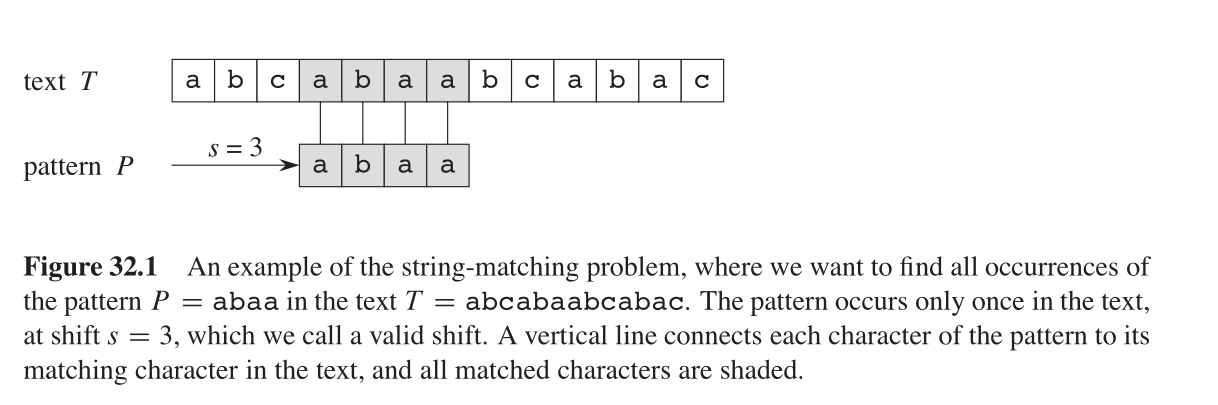
\includegraphics[width=350pt]{main--string-matching-4d75.png} 

 \begin{itemize}
 \item Hvis mønsteret $P$ forekommer med shift $s$ i $T$, kalder vi $s$ et \textbf{valid shift}, og ellers et \textbf{invalid shift}.
 \item String matching problemet er problemet om at finde \textbf{alle} valide shifts givet et mønster $P$ der forekommer i tekst $T$.
 \end{itemize}
\end{frame}

\begin{frame}
  \frametitle{Oversigt over string-matching algoritmer}
  
  \begin{table}[]
\centering
\begin{tabular}{lll}
\toprule
\textbf{Algorithm}          & \textbf{Preprocessing Time} & \textbf{Matching Time} \\
\midrule
\textit{Naive}              & $0$                         & $O((n-m+1)m)$          \\
\textit{Rabin-Karp}         & $\Theta (m)$                & $O((n-m+1)m)$          \\
\textit{Finite Automaton}   & $O(m |\Sigma |)$            & $\Theta (n) $          \\
\textit{Knuth-Morris-Pratt} & $\Theta (m)$                & $\Theta (n)$           \\
\bottomrule
\end{tabular}
\end{table}
\end{frame}

\begin{frame}[allowframebreaks]
  \frametitle{Preprocessing}
 \begin{itemize}
 \item Alle algoritmer med undtagelse af den naive laver noget preprocessing baseret på et mønster og finder så alle valide shifts. 
 \item At finde de valide shifts kalder vi ``matching''
 \item Rabin Karp har en langt bedre average-case på trods af at dens worst case er det samme som naiv.
 \end{itemize} 
\end{frame}

\begin{frame}[allowframebreaks]
  \frametitle{Terminologi}
 \begin{itemize}
 \item Vi betegner sættet af alle endelige strenge formet af alfabetet $\Sigma$ som værende $\Sigma^*$
 \item Bemærk at $\varepsilon$ (den tomme streng) også er en del af $\Sigma^{*}$.
 \item Længden af en streng, $x$ bliver betegnet som $|x|$
 \item Concatenation bliver betegnet som $xy$ og har længden $|x| + |y|$. Der er, simpelt, karaktererne i $x$ efterfulgt af karaktererne i $y$.
   \item Vi siger at $\omega$ er et præfix af en streng $x$, betegner $\omega \sqsubset x$, hvis $x = \omega y, y \in \Sigma^{*}$. 
   \item Bemærk at hvis $\omega \sqsubset x$, så $|w| \leq |x|$. 
   \item Endvidere siger vi at $\omega$ er et suffix af en streng $x$, betegnet $x \sqsupset x$, hvis $x = y \omega$ for en $y \in \Sigma^{*}$. 
   \item Som med et præcis, hvis $w \sqsupset x$ så $|\omega| \leq |x|$.
   \item Bemærk også at $\sqsubset $ og $\sqsupset$ er transitive relationer. 
 \end{itemize} 
 \begin{lemma}[31.1 (Overlapping-suffic lemma)]
Suppose that $x, y, $ and $z$ are strings such that $x \sqsupset z$ and $y \sqsupset z$. If $|x| \leq |y|$, then $x \sqsupset y$. If $|x| \geq |y|$, then $y \sqsupset x$. If $|x| = |y|$, then $x = y$.
\end{lemma}
\begin{itemize}
\item Vi bruger et grafisk bevis:
\end{itemize}
\vspace{1cm}
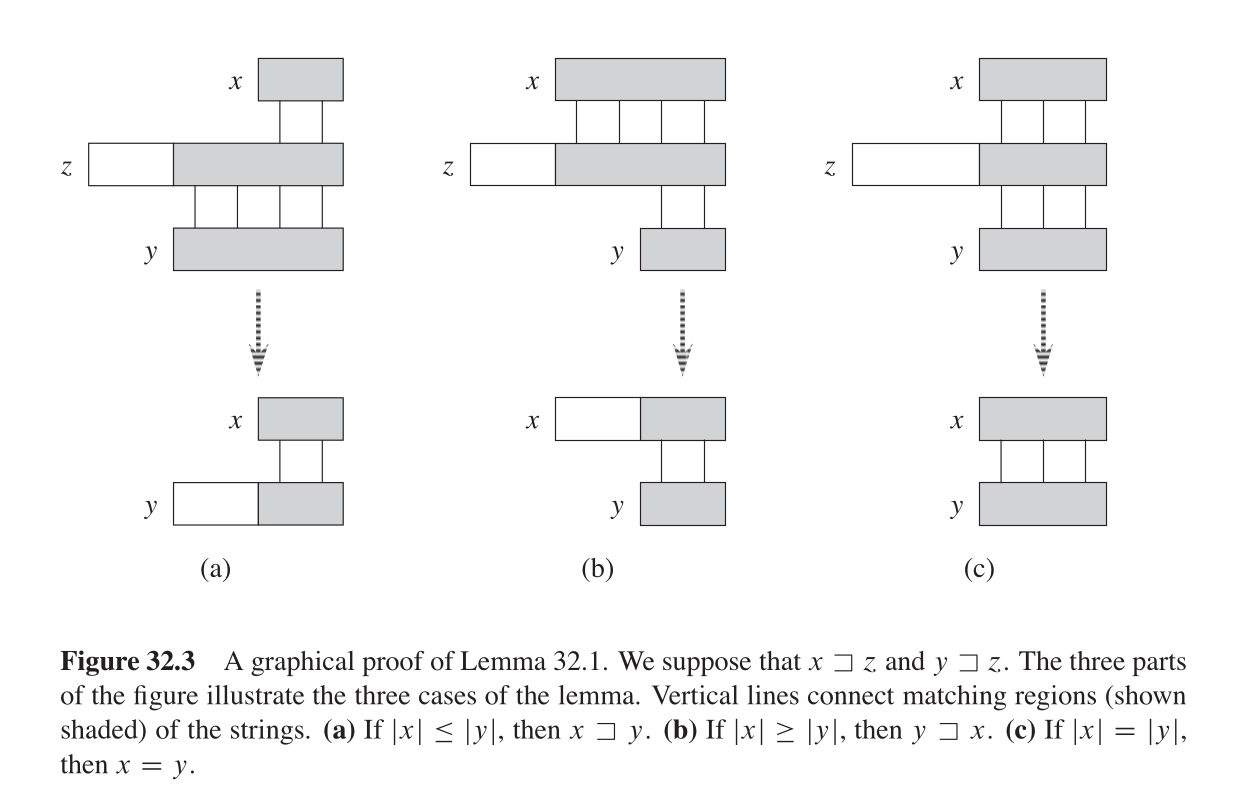
\includegraphics[width=330pt]{main--string-matching-c1c3.png}
\vspace{1cm}

\end{frame}

\begin{frame}[allowframebreaks]
  \frametitle{Terminologi}
  
\begin{itemize}
\item For lethed af notation, betegner vi en $k$-karakters præfix $P[1..k]$ af møsteret $P[1..m]$ af $P_{k}$. Dermed $P_{0} = \varepsilon$, $P_{m} = P = P[1..M]$ (så længe man går ud fra at længden af $P$ er $m$.)
\item Ved brug af denne notation kan vi sige at string-matching problemet er det hvor vi skal finde alle shifts $s$ i rangen $0 \leq s \leq n -m$ således at $P \sqsupset T_{s+m}$.
\item I den pseudokode vi kommer til at bruge, tillader vi to strenge på samme længde til at blive sammenlignet som en primitiv operation (som +, - etc).
\item Hvis strengene bliver sammenlignet venstre til højre og sammenlignningen stopper når et mismatch er fundet, kan vi assume at tiden taget er en lineær funktion af antallet af sammenlignet karakterer fundet. 
\item Så, for at være præcis, testen \texttt{x == y} er antaget at tage tiden $\Theta (t+1)$, hvor $t$ er længden af den længste streng $z$, således at $z \sqsubset x$, og $z \sqsubset y$. (Vi skriver $\Theta (t+1)$ i stedet for $\Theta(t)$ for at kunne tage den case hvor $t = 0$)
\end{itemize}
\end{frame}

\section{The Naive String-Matching Algorithm}
\label{sec:label}


\begin{frame}
  \frametitle{Den Naive String-Matching Algorithme}
  \begin{itemize}
  \item Den naive (brute-force) string-matching algoritme finder alle valide shifts ved brug at et loop. 
  \item Loopet tjekker condition $P[1..m] = T[s+1 .. s+m]$ for hver linje af de $n-m+1$ mulige værdier a $s$. 
  \end{itemize}
  
  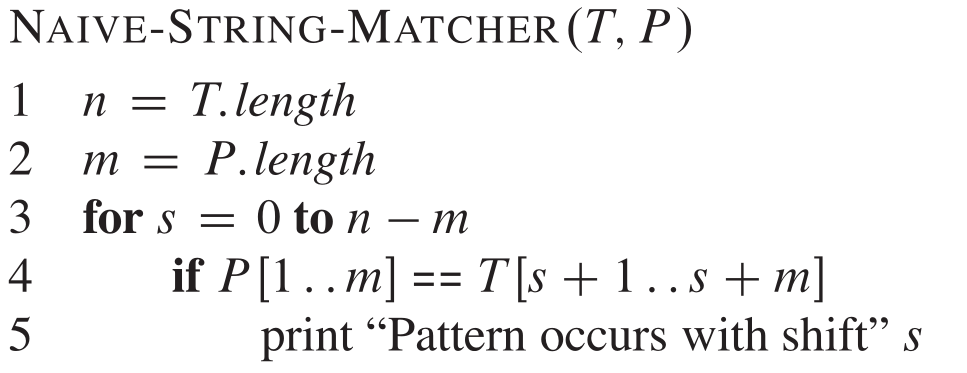
\includegraphics[width=300pt]{main--the-naive-string-matching-algorithm-3b93.png}
\end{frame}

\begin{frame}[allowframebreaks]
  \frametitle{Naive Approach}
  \begin{itemize}
  \item Køretiden på denne algoritme er $O((n-m+1)m)$ hvilket er ret lort. 
  \item Det kan blive $\Theta (n^{2})$ hvis vi har en streng $a^{n}$ og et mønster $a^{m}$, og $m = \lfloor n / 2 \rfloor$. 
  \item Til gengæld ingen preprocessing!
  \end{itemize}
\end{frame}

\subsection{Rabin-Karp}
\label{subsec:label}



\begin{frame}[allowframebreaks]
  \frametitle{Rabin-Karp}
  \begin{itemize}
    \item Randomiseret algoritme, dog bliver den først beskrevet uden randomisering
    \item Idé: Tænk på $P$ og $T$ som værende tal og sammenlign $P$ og $T_{s+1..s+m}$ ved at sammenligne tallene
    \item Vi kører i radix-$d$ hvor $d = |\Sigma|$. 
    \item Det betyder at vi bruger tallene i base-$d$.
    \item Mere notation!:
    \item $p$ (lille $p$): Decimalværdien af $P[1..m]$
    \item $t_{s}$: Decimalværdien af $T[s+1..s+m]$
    \item Dermed, hvis $p = t_{s}$ har vi et \textbf{match}!
    \item \textbf{Antagelse}: Størrelsen af tallene $p$ og $t$ er ikke så store at deres lighed ikke kan findes i konstant tid.
    \item Hvordan finder vi så værdien af $p$?
  \end{itemize}
\end{frame}

\begin{frame}[allowframebreaks]
  \frametitle{Horner's Rule og udregning af tal}
  \begin{itemize}
  \item Horners rule er en regneregel til at finde værdien af store tal hurtigt, specielt hurtigt i computere. 
  \end{itemize}
  \begin{center}
    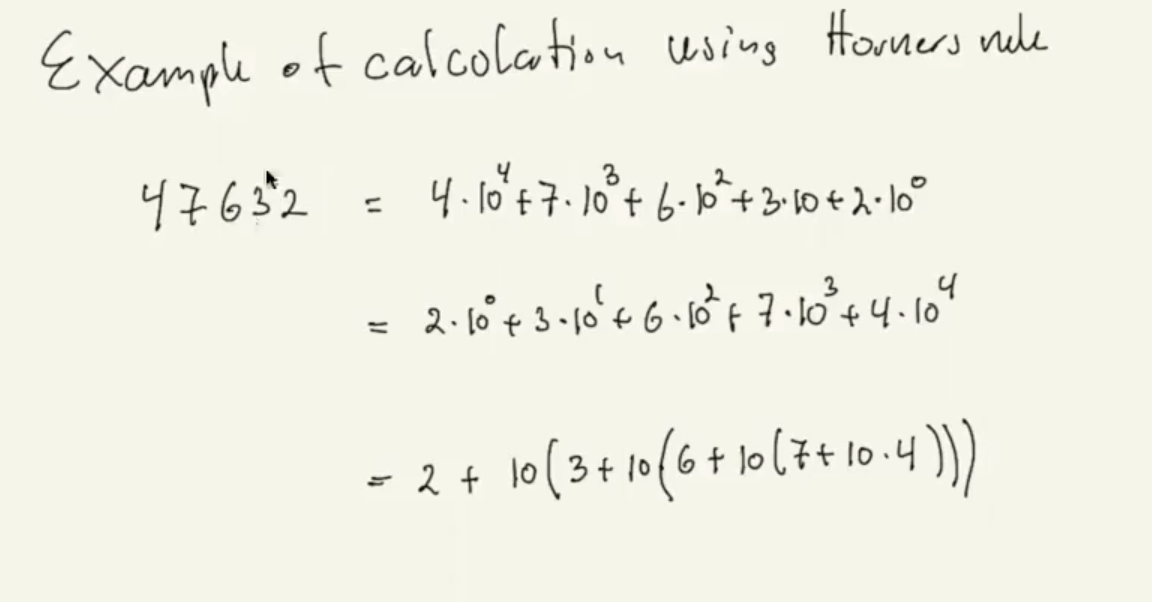
\includegraphics[width=300pt]{main--the-naive-string-matching-algorithm--rabin-karp-c553.png} 
  \end{center}
  \begin{itemize}
  \item Dermed: $p = P[m] + 10(P[m-1] + 10(P[m-2]+ \cdots + 10(P[i])\cdots))$
  \item På samme måde er $t_{0}$ udregnet fra $T[1..m]$ i $\Theta(m)$
  \item Vi kan hurtigt udregne $t_{s+1}$ fra $t_{s}$ da $t_{s+1} = 10(t_{s}-10^{m-1}T[s+1])+T[s+m+1]$
  \end{itemize}
  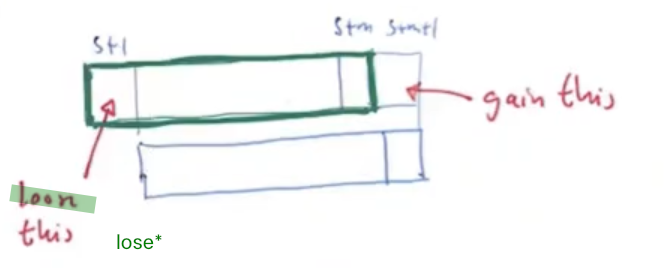
\includegraphics[width=300pt]{main--the-naive-string-matching-algorithm--rabin-karp-44af.png}
  \begin{itemize}
  \item Det tager $O(1)$ konstant tid er udregne det næste $t_{s+1}$, når $10^{m-1}$ er udregnet tidligere, som tager $O(m)$ tid (men, som vi ser senere, kan blive gjort i $O(\log m)$ tid.
  \end{itemize}
\end{frame}

\begin{frame}[fragile]
  \frametitle{Rabin-Karp}
  \begin{verbatim}
Compute p in time O(m)
Compute t_0 in time O(m) - report match if p = t_0
Compute t_1 in time O(1) - Report match if p = t_1
.
.
.
Compute t_(n-m) in time O(1) - Report match if p = t_(n-m)
\end{verbatim}
\end{frame}

\begin{frame}[allowframebreaks]
  \frametitle{Rabin-Karp}
 \begin{itemize}
 \item Total tid: $\Theta(m)$ preprocessing (konvertering til tal)
 \item $\Theta(n-m+1)$ matching tid.
 \item Det er dog too-good-to-be-true:(
 \item Hvad hvis $p$ er for stort til at vi kan sammenligne i konstant tid?
 \end{itemize} 
\end{frame}

\begin{frame}[allowframebreaks]
  \frametitle{Løsning til køretidsproblemet}
  \begin{itemize}
  \item Vi løser dette problem ved at udregne $p$ og $t_{s}$ modulo $q$.
  \item Vi kan udregne $p \mod q$ i $\Theta(m)$, $t_{0} \mod q$ i $\Theta(m)$
  \item \textbf{Hvordan finder vi en god værdi af $q$}?
  \item Så stort som muligt. $10q$ skal gerne være værdien af et \texttt{word}.
  \item $10q$ fordi vi gerne vil kunne lave udregningen v.h.a Horner's Rule. 
  \item Ved et generelt alfabet: 
  \end{itemize}
  \begin{theorem}
    $\Sigma = \{0,1,2,\ldots, d-1\}$
    Chose $q$ such that $dq$ fits in one computer word.
    $t_{s+1} = (d(t_{s}-T[s+1] \cdot h) + T[s+m+1]) \mod q$
    when $h = d^{m-1} \mod q$
  \end{theorem}
  \begin{itemize}
  \item Nyt problem: 
  \item ``Spurious Hits'' $t_{s} \equiv p \mod q$ men $t_{s} \neq p$: 
  \item Vi gider ikke de hits! >:(
  \item Vi skal derfor teste alle shifts med $t_{s} \equiv p \mod q$
  \item Det er $\Theta(m)$ per test.
  \item Dermed bliver worst case matching tid en del værre: $\Theta((n-m+1)m)$
  \end{itemize}
\end{frame}

\begin{frame}[allowframebreaks]
  \frametitle{Forventede antal hits}
  
  \begin{itemize}
  \item Antag at $\mod q$ agerer som en tilfældig mapping fra alfabetet til hele tal base q, i.e., $\Sigma^{*} \rightarrow \mathbb{Z}_{q}$
  \item Hvis vi antager at alle værdierne $\mod q$ er lige sandsynlige, så $p(t_{s} \equiv p \mod q)= \frac{1}{q}$
  \item Så er antallet af ``spurious hits'', i.e., hits vi ikke vil have (falske), $\frac{O(n)}{q} = O(\frac{n}{q})$
  \item Nu når vi ved det, kan vi så finde den forventerede matchingtid (køretid).
  \end{itemize}
\end{frame}

\begin{frame}[allowframebreaks]
  \frametitle{Forventede køretid}
  \begin{itemize}
  \item $O(n) + O(m(v + \frac{n}{q}))$
  \item Hvor $v$ er antallet af korrekte hits
  \item Og $v$ er $O(1)$ og $q \geq m$.
  \item Tiden på dette er $O(n)$
  \item So den totale tid (med preprocessing og matches) er $O(n+m) = O(n)$ da $n \geq m$
  \item Yippeee!
  \end{itemize}
\end{frame}

\subsection{String matching with DFA's}
\label{subsec:label}

\begin{frame}[allowframebreaks]
  \frametitle{String matching med DFA's}
  \begin{itemize}
  \item Vi kan også matche strings med DFA'er.
  \item Jeg går ikke over de helt basale definitioner. 
  \item Vi siger at en endelig maskine $M$ accepterer $w \in \Sigma^{*}$ hvis, når maskinen har kørt $w$ igennem (spist, ifølge Jørgen), og den sidste state er en accept state. 
  \item $M$ accepterer \textbf{ikke} $w \in \Sigma^{*}$ hvis den ikke ender i en accepting state.
  \item Vi definerer $\phi$ til at være \textbf{final state funktionen}, som er den state $M$ er i efter den har spist $w$. 
  \item Så hvis $\phi(w) \in A$ hvor $A$ er sættet af accepting states, så accepterer vi $w$.
  \item Vi vil nu bygge en automata lavet til string matching, innovativt nok, kalder vi den for \textbf{string matching automata}.
  \end{itemize}
\end{frame}

\begin{frame}[allowframebreaks]
  \frametitle{String Matching Automata}
  \begin{itemize}
  \item \textbf{Mål}: $M$ accepterer hvert præfix $T_{s+m}$ af en tekst $T$ hvor de sidste $m = |P|$ karakterer af $T_{s+m}$ er lig $p$.
  \item Notationstid!
  \item \textbf{Suffix Funktion} for mønster $p$:
  \item $\sigma : \Sigma^{*} \rightarrow \{ 0,1,2 \ldots, m \} $
  \item $\sigma(x) = \text{max}\{k | P_{k} \sqsupset x\}$
  \item $\sigma$ er \textit{well-defined} da $\varepsilon \sqsupset x\;\; \forall x \in \Sigma^{*}$
  \item Well-defined, da der er et værdi for hvert input.
  \end{itemize}
  \begin{lemma}[32.2]
$\forall x \in \Sigma^{*}, a \in \Sigma \;\;\;\;\; \sigma(xa) \leq \sigma(x)+1$
  \end{lemma}
  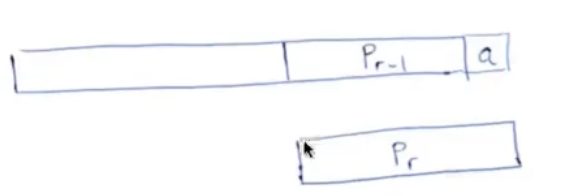
\includegraphics[width=300pt]{main--the-naive-string-matching-algorithm--string-matching-with-dfa's-6ee3.png}
  \begin{itemize}
  \item Så er det tid til at definere \textit{string matching automaton}!
  \item $M = M(p)\;\;\;\;p=P[1..m]$
  \item Givet at længden af mønstret $p$ har længde $m$, i så fald vil $M$ have states $Q = \{0, 1, 2, \ldots, m\}, q_{0} = 0, A = \{m\}$
  \item $\sigma (q,a) = \sigma_{q}(P_{a})$
  \item Vi vælger $\sigma$ så, hvis automataen er i state q, så er den nuværrende streng $T_{i}$ satisfier at $P_{q} \sqsupset T_{i}$ og $q = \sigma(T_{i})$
  \item I.e., når der er spist $T_{i}$, så skal $P_q \sqsupset T_{i}$ og $q$ den længste suffiks af $T_{i}$.
  \end{itemize}
\end{frame}



\end{document}